% ============================================================
% RESULTS (part B): GAN augmentation and GAN anomaly detection
% ============================================================
\subsection{Augmentation under Scarcity: Does the GAN Help? (E3)}

This experiment asks the question that motivated the use of a GAN: if only a handful of real faulty programs are available
per class, do synthetic feature vectors improve the classifier? Figure~\ref{fig:augment} and
Tables~\ref{tab:augrf}--\ref{tab:augmlp} give the test macro-F1 of the seven regimes, averaged over ten seeds. The
\emph{valid} class always has 400 real training programs.

\begin{figure}[H]
\centering
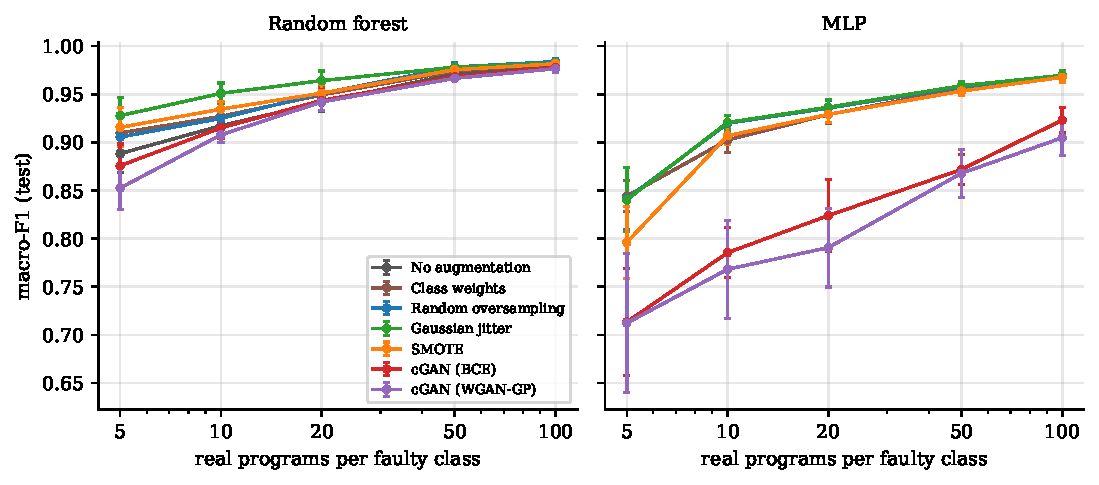
\includegraphics[width=\textwidth]{figs/augment.pdf}
\caption{Test macro-F1 against the number of real training programs per faulty class (mean $\pm$ standard deviation over ten
seeds). Left: random forest. Right: MLP.}
\label{fig:augment}
\end{figure}

\begin{table}[H]
\centering
\caption{Random forest: test macro-F1 (mean $\pm$ s.d., ten seeds) against the number of real programs per faulty class.
Bold marks the best mean in each column.}
\label{tab:augrf}
\small
\resizebox{\textwidth}{!}{\begin{tabular}{lccccc}
\toprule
\textbf{Method} & \textbf{5} & \textbf{10} & \textbf{20} & \textbf{50} & \textbf{100}\\
\midrule
No augmentation & 0.888\,$\pm$\,0.020 & 0.917\,$\pm$\,0.009 & 0.942\,$\pm$\,0.009 & 0.971\,$\pm$\,0.003 & 0.979\,$\pm$\,0.003\\
Class weights & 0.910\,$\pm$\,0.018 & 0.927\,$\pm$\,0.008 & 0.949\,$\pm$\,0.008 & 0.974\,$\pm$\,0.004 & 0.982\,$\pm$\,0.003\\
Random oversampling & 0.906\,$\pm$\,0.020 & 0.925\,$\pm$\,0.010 & 0.951\,$\pm$\,0.009 & \textbf{0.978\,$\pm$\,0.004} & \textbf{0.984\,$\pm$\,0.003}\\
Gaussian jitter & \textbf{0.928\,$\pm$\,0.019} & \textbf{0.951\,$\pm$\,0.011} & \textbf{0.964\,$\pm$\,0.010} & 0.978\,$\pm$\,0.002 & 0.982\,$\pm$\,0.003\\
SMOTE & 0.916\,$\pm$\,0.020 & 0.935\,$\pm$\,0.008 & 0.951\,$\pm$\,0.009 & 0.975\,$\pm$\,0.005 & 0.982\,$\pm$\,0.003\\
cGAN (BCE) & 0.876\,$\pm$\,0.023 & 0.915\,$\pm$\,0.011 & 0.944\,$\pm$\,0.011 & 0.968\,$\pm$\,0.003 & 0.978\,$\pm$\,0.003\\
cGAN (WGAN-GP) & 0.853\,$\pm$\,0.022 & 0.908\,$\pm$\,0.008 & 0.942\,$\pm$\,0.009 & 0.967\,$\pm$\,0.001 & 0.977\,$\pm$\,0.004\\\bottomrule
\end{tabular}
}
\end{table}

\begin{table}[H]
\centering
\caption{MLP: same protocol as Table~\ref{tab:augrf}.}
\label{tab:augmlp}
\small
\resizebox{\textwidth}{!}{\begin{tabular}{lccccc}
\toprule
\textbf{Method} & \textbf{5} & \textbf{10} & \textbf{20} & \textbf{50} & \textbf{100}\\
\midrule
No augmentation & \textbf{0.844\,$\pm$\,0.016} & 0.902\,$\pm$\,0.013 & 0.929\,$\pm$\,0.009 & 0.956\,$\pm$\,0.005 & 0.969\,$\pm$\,0.004\\
Class weights & \textbf{0.844\,$\pm$\,0.016} & 0.902\,$\pm$\,0.013 & 0.929\,$\pm$\,0.009 & 0.956\,$\pm$\,0.005 & 0.969\,$\pm$\,0.004\\
Random oversampling & 0.842\,$\pm$\,0.032 & 0.920\,$\pm$\,0.008 & 0.936\,$\pm$\,0.008 & 0.958\,$\pm$\,0.005 & \textbf{0.970\,$\pm$\,0.005}\\
Gaussian jitter & 0.840\,$\pm$\,0.033 & \textbf{0.921\,$\pm$\,0.007} & \textbf{0.936\,$\pm$\,0.008} & \textbf{0.959\,$\pm$\,0.004} & 0.970\,$\pm$\,0.005\\
SMOTE & 0.796\,$\pm$\,0.038 & 0.907\,$\pm$\,0.010 & 0.929\,$\pm$\,0.008 & 0.953\,$\pm$\,0.005 & 0.968\,$\pm$\,0.005\\
cGAN (BCE) & 0.713\,$\pm$\,0.055 & 0.785\,$\pm$\,0.026 & 0.824\,$\pm$\,0.038 & 0.872\,$\pm$\,0.016 & 0.923\,$\pm$\,0.013\\
cGAN (WGAN-GP) & 0.712\,$\pm$\,0.073 & 0.768\,$\pm$\,0.051 & 0.791\,$\pm$\,0.041 & 0.868\,$\pm$\,0.025 & 0.905\,$\pm$\,0.018\\\bottomrule
\end{tabular}
}
\end{table}

\paragraph{The short answer is no.} With the random forest, the conditional GAN is never the best method and is usually
within noise of using no augmentation at all: at 20 real programs per class the BCE version scores 0.944 against 0.942 without
augmentation, and at 5 programs it is \emph{worse} (0.876 and 0.853 for the BCE and WGAN-GP versions, against 0.888). The
cheap alternatives help more. Gaussian jitter is the best method at every size up to 20 programs per class (0.928 against
0.888 at five programs), and SMOTE, random oversampling and class weights also give small gains. By 100 programs per class
all methods are within one point of each other. For the MLP the picture is worse for the GAN: its synthetic vectors cost
between 5 and 13 points of macro-F1 relative to no augmentation, with the largest damage at the smallest sizes
(0.713 against 0.844 at five programs per class), presumably because the MLP, unlike a forest, tries to fit every synthetic point.

Table~\ref{tab:augtests} gives paired comparisons over the ten seeds. The difference between the GAN and \emph{no augmentation}
is small and, depending on the size, indistinguishable from zero or slightly negative; the difference from jitter and SMOTE is
negative at every size. The $p$-values are uncorrected for the 30 comparisons shown, so they should be read as a rough guide.

\begin{table}[H]
\centering
\caption{Paired difference in macro-F1 (random forest) between each GAN and three alternatives, with the two-sided
paired $t$-test $p$-value in parentheses. Negative values mean the GAN is worse.}
\label{tab:augtests}
\small
\resizebox{\textwidth}{!}{\begin{tabular}{rlccc}
\toprule
\textbf{Real/class} & \textbf{GAN} & \textbf{vs.\ none} & \textbf{vs.\ SMOTE} & \textbf{vs.\ jitter}\\
\midrule
5 & cGAN (BCE) & -0.013 (0.034) & -0.040 (0.001) & -0.052 (0.001)\\
5 & cGAN (WGAN-GP) & -0.036 (0.007) & -0.063 (0.000) & -0.075 (0.000)\\
10 & cGAN (BCE) & -0.002 (0.163) & -0.019 (0.004) & -0.036 (0.000)\\
10 & cGAN (WGAN-GP) & -0.010 (0.016) & -0.027 (0.000) & -0.043 (0.000)\\
20 & cGAN (BCE) & +0.002 (0.378) & -0.008 (0.013) & -0.021 (0.000)\\
20 & cGAN (WGAN-GP) & +0.000 (0.920) & -0.009 (0.000) & -0.022 (0.000)\\
50 & cGAN (BCE) & -0.003 (0.010) & -0.008 (0.000) & -0.010 (0.000)\\
50 & cGAN (WGAN-GP) & -0.005 (0.001) & -0.009 (0.000) & -0.012 (0.000)\\
100 & cGAN (BCE) & -0.001 (0.015) & -0.004 (0.000) & -0.004 (0.000)\\
100 & cGAN (WGAN-GP) & -0.003 (0.002) & -0.005 (0.000) & -0.006 (0.000)\\\bottomrule
\end{tabular}
}
\end{table}

\paragraph{Where the benefit of augmentation lies.} Figure~\ref{fig:augclass} breaks the result down by class for 20 real
programs per class. Most classes are already close to their ceiling without help. The exception is \emph{logic}, the family whose
members are partly invisible to the compiler and have to be recognised from the six pattern features: with five real programs
its F1 is 0.52 without augmentation, 0.79 with jitter, 0.70 with SMOTE and 0.47 with the BCE GAN; at 20 programs the values are
0.82, 0.93, 0.86 and 0.85. Augmentation in this setting is mostly a regulariser for the one hard class. The valid class
gains as a side effect, because fewer logic programs are mistaken for it.

\begin{figure}[H]
\centering
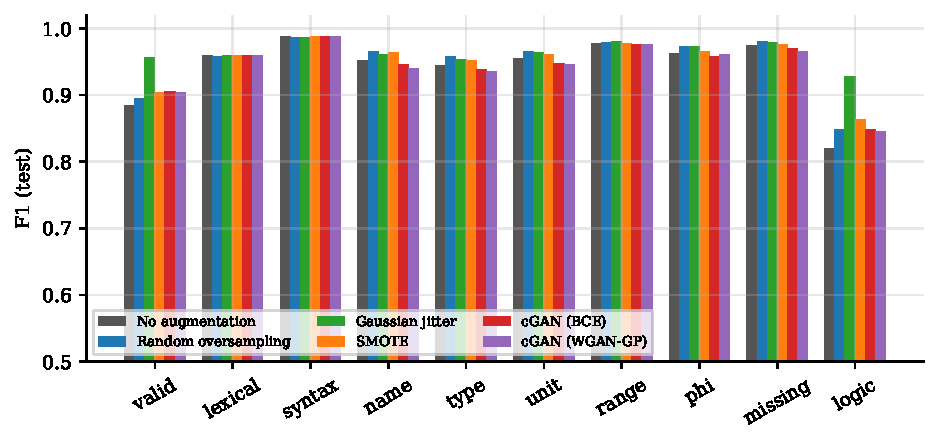
\includegraphics[width=\textwidth]{figs/augment_perclass.pdf}
\caption{Per-class F1 of the random forest with 20 real programs per faulty class (mean of ten seeds).}
\label{fig:augclass}
\end{figure}

\paragraph{Why the GAN fails: fidelity of the synthetic vectors.} For one seed at 20 programs per class we checked
the synthetic vectors directly (Table~\ref{tab:fidelity}). \emph{Label validity} is the fraction of synthetic vectors that an
oracle random forest, trained on the full 8{,}000-program pool, assigns to the class the generator was asked for. \emph{NN distance}
is the mean standardised distance to the nearest real training vector of that class; for reference, held-out \emph{real}
programs of the same classes lie at a mean distance of \HeldoutNN{} from their nearest training example.

\begin{table}[H]
\centering
\caption{Fidelity of synthetic vectors (seed 0, 20 real programs per faulty class). Label validity for the three resampling methods is
high by construction: their points lie on or next to real training vectors that the oracle has itself seen.}
\label{tab:fidelity}
\small
\begin{tabular}{lrrr}
\toprule
\textbf{Generator} & \textbf{Label validity} & \textbf{NN distance} & \textbf{Exact copies (\%)}\\
\midrule
Random oversampling & 1.000 & 0.00 & 100.0\\
Gaussian jitter & 1.000 & 0.84 & 0.0\\
SMOTE & 1.000 & 3.01 & 0.0\\
cGAN (BCE) & 0.037 & 11.30 & 0.0\\
cGAN (WGAN-GP) & 0.043 & 10.80 & 0.0\\\bottomrule
\end{tabular}

\end{table}

The result is stark. Only 4\% of the GAN's vectors are recognised as belonging to the requested class, which is below the
10\% expected from a classifier guessing among ten classes; the GAN vectors are also \emph{further} from the training data than genuinely
new real programs are. In other words, the generator has not learned the class-conditional structure. Figure~\ref{fig:pca} shows the same thing
in two dimensions: the synthetic points (crosses) spread over the whole cloud of all classes instead of concentrating where the real
examples of the requested class lie, although a two-dimensional projection of mostly discrete count features is only a rough picture.

\begin{figure}[H]
\centering
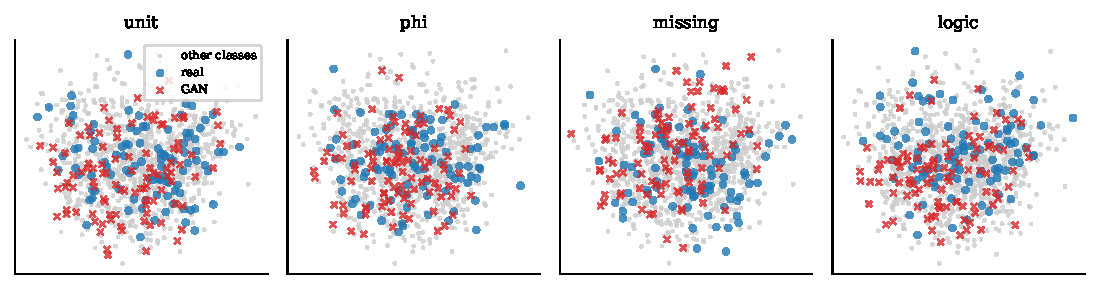
\includegraphics[width=\textwidth]{figs/gan_pca.pdf}
\caption{PCA projection of real (circles) and GAN-generated (crosses) vectors for four classes, with all other real vectors in grey
(a GAN trained on 100 real programs per class).}
\label{fig:pca}
\end{figure}

We examined one likely cause. In the experiment above, mini-batches were drawn uniformly from the training set, which is dominated by the
400 \emph{valid} programs, so each rare class contributed only a few percent of the batches and the generator may have learned to ignore its
class input. We repeated the experiment (five seeds, 20 real programs per class) with class-balanced mini-batches, in which a class is chosen
first and an example second. Table~\ref{tab:gandiag} shows the outcome: label validity rises from roughly 4\% to 11--13\%, which is
about chance level, and macro-F1 does not improve. The imbalance in the batches therefore explains part of the failure but not the
rest. The remaining explanation is the one the numbers suggest: with 20 examples per class in a 101-dimensional space of counts,
a small unregularised GAN has too little to learn from, and a continuous generator blurs features that carry discrete, tightly coupled
meaning (for example, a diagnostic count of one for exactly one code). This follows the pattern commonly reported for GANs trained on very small tabular data, and it is a
limit of our setup rather than a general statement about GANs. We did not test architectures designed for tabular data, such as CTGAN
\cite{xu2019}, or any hyper-parameter search.

\begin{table}[H]
\centering
\caption{Effect of class-balanced mini-batches on the GAN (20 real programs per faulty class; mean $\pm$ s.d. over five seeds).
Label validity of about 0.10 is chance level.}
\label{tab:gandiag}
\small
\begin{tabular}{llcc}
\toprule
\textbf{Model} & \textbf{Mini-batches} & \textbf{Label validity} & \textbf{Macro-F1}\\
\midrule
cGAN (BCE) & uniform & 0.039\,$\pm$\,0.023 & 0.944\,$\pm$\,0.011\\
cGAN (WGAN-GP) & uniform & 0.045\,$\pm$\,0.005 & 0.944\,$\pm$\,0.008\\
cGAN (BCE) & class-balanced & 0.110\,$\pm$\,0.011 & 0.943\,$\pm$\,0.009\\
cGAN (WGAN-GP) & class-balanced & 0.126\,$\pm$\,0.009 & 0.935\,$\pm$\,0.010\\\bottomrule
\end{tabular}

\end{table}

\paragraph{What the GAN is and is not good for here.} One property is worth noting: none of the synthetic vectors is an exact copy of a
real one (0\% exact copies in Table~\ref{tab:fidelity}), whereas random oversampling copies by definition. If privacy were the
goal, that would matter; but a synthetic set that does not carry the class signal is no use as training data either. Our
evidence supports a narrow conclusion: \emph{in this setting, with these model sizes and this amount of data, simple resampling
is the better way to handle rare error classes.}

\subsection{GAN-Based Anomaly Detection (E4)}

The second use of a GAN is to detect faulty programs when no faulty examples are available at all. A GAN is trained on the 800 valid
training programs; the negated discriminator output is the anomaly score. Table~\ref{tab:anomaly} and Figure~\ref{fig:anomaly}
give the AUROC of each detector separating the 200 valid test programs from the 200 programs of each faulty family.

\begin{figure}[H]
\centering
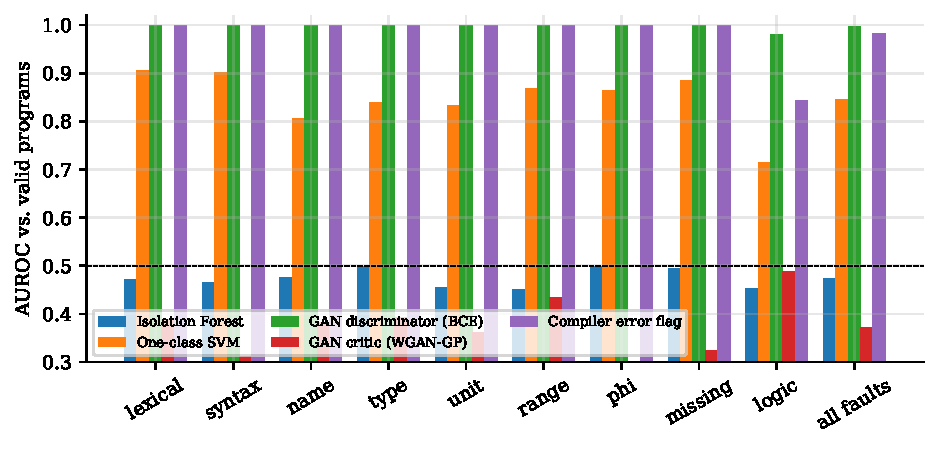
\includegraphics[width=\textwidth]{figs/anomaly.pdf}
\caption{AUROC of five detectors for valid versus faulty programs, by fault family (dashed line: chance).}
\label{fig:anomaly}
\end{figure}

\begin{table}[H]
\centering
\caption{AUROC of valid-versus-faulty detection by fault family. All detectors except the compiler flag were trained on
valid programs only.}
\label{tab:anomaly}
\small
\resizebox{\textwidth}{!}{\begin{tabular}{lrrrrr}
\toprule
\textbf{Fault family} & \textbf{Isolation Forest} & \textbf{One-class SVM} & \textbf{GAN discriminator (BCE)} & \textbf{GAN critic (WGAN-GP)} & \textbf{Compiler error flag}\\
\midrule
lexical & 0.471 & 0.905 & 1.000 & 0.388 & 1.000\\
syntax & 0.465 & 0.901 & 1.000 & 0.310 & 1.000\\
name & 0.475 & 0.806 & 1.000 & 0.381 & 1.000\\
type & 0.498 & 0.839 & 1.000 & 0.392 & 1.000\\
unit & 0.454 & 0.834 & 1.000 & 0.360 & 1.000\\
range & 0.451 & 0.867 & 1.000 & 0.433 & 1.000\\
phi & 0.498 & 0.865 & 1.000 & 0.265 & 1.000\\
missing & 0.495 & 0.885 & 1.000 & 0.325 & 1.000\\
logic & 0.452 & 0.715 & 0.981 & 0.487 & 0.843\\
all faults & 0.473 & 0.846 & 0.998 & 0.371 & 0.982\\\bottomrule
\end{tabular}
}
\end{table}

The numbers need careful reading, because the headline is easy to over-interpret.

\begin{itemize}
    \item \textbf{The BCE discriminator is an excellent detector, but most of that is easy.} It reaches an AUROC of 0.998 over all faults. However,
    49 of the 101 features, including \emph{all} 40 diagnostic features, are constant on valid programs: a valid program reports no diagnostic. Any
    model that looks at those features can therefore tell a program with an error from one without. The compiler's own ``at least one error'' flag
    achieves 1.000 on every family except \emph{logic}, and it is a far simpler detector.
    \item \textbf{The informative column is \emph{logic}.} There the compiler flag falls to 0.843 (the soft faults raise no diagnostic), the one-class
    SVM reaches 0.715, and the BCE discriminator 0.981. To check that this is not a lucky seed, we retrained the discriminator with five seeds
    (Table~\ref{tab:anomalycheck}): the logic AUROC is 0.97--0.99 each time. It depends, however, on the pattern features: without them it drops to
    0.83--0.87, and the pattern features alone give only 0.60--0.69. So the discriminator's advantage comes from combining the
    compiler-derived signals with the pattern signal that valid programs never exhibit, and the pattern features were written with this fault in mind.
    \item \textbf{Isolation Forest is at chance (0.47).} We first suspected that it ignores the diagnostic features because they have zero range on the
    training data, so a random split cannot use them. Removing the constant features altogether changes nothing (0.473 to 0.475), which is consistent with that
    explanation: among the features that do vary, faulty programs look like valid ones.
    \item \textbf{The WGAN-GP critic fails.} Its AUROC is 0.37, \emph{below} chance: faulty programs receive a higher critic value than valid ones. A critic is
    trained to separate real from generated samples, not to model density, and outside the data it extrapolates. Negating the score would give about 0.63, but we report the
    score as defined in advance, not a sign chosen after seeing the result.
\end{itemize}

\begin{table}[H]
\centering
\caption{Stability and ablation of the BCE discriminator as anomaly detector (five seeds, mean $\pm$ s.d.).}
\label{tab:anomalycheck}
\small
\begin{tabular}{lcc}
\toprule
\textbf{Discriminator input} & \textbf{AUROC, logic} & \textbf{AUROC, all faults}\\
\midrule
All 101 features & 0.978\,$\pm$\,0.008 & 0.996\,$\pm$\,0.003\\
Without pattern features & 0.844\,$\pm$\,0.015 & 0.982\,$\pm$\,0.001\\
Pattern features only & 0.620\,$\pm$\,0.034 & 0.521\,$\pm$\,0.025\\\bottomrule
\end{tabular}

\end{table}

The practical reading is modest. A GAN discriminator trained only on valid programs is a usable \emph{unsupervised} detector of the one family that the compiler
misses, but it is not better than the compiler on the families the compiler handles, and its result is only as good as the features it sees.
